\documentclass[border=3pt]{standalone}
% Preâmbulo compartilhado pelos diagramas TikZ da aula
\usepackage[T1]{fontenc}
\usepackage[utf8]{inputenc}
\usepackage{lmodern}
\usepackage{amsmath}
\usepackage{xcolor}
\usepackage{tikz}
\usetikzlibrary{arrows.meta,angles,quotes,decorations.pathmorphing,calc,
                positioning,shapes.geometric,backgrounds,fit}

% Paleta (mesma dos SVGs originais)
\definecolor{dblue}{HTML}{2A5B8C}
\definecolor{dorange}{HTML}{B3541E}
\definecolor{dgreen}{HTML}{4A7C59}
\definecolor{dred}{HTML}{9C4B4B}
\definecolor{dcream}{HTML}{F4F1EA}
\definecolor{dshade}{HTML}{DDD7C9}

% Estilos comuns (prefixo d... para não colidir com chaves internas do pgf)
\tikzset{
  >={Stealth[length=2mm]},
  dguide/.style={gray!55, dashed, line width=0.4pt},
  daxis/.style={gray!60, line width=0.7pt, ->},
  dbody/.style={fill=black!3, draw=black!80, line width=1pt},
  dacc/.style={draw=dblue, line width=1pt},
  dlbl/.style={black!55, font=\small},
  dsub/.style={black!45, font=\footnotesize},
  dstate/.style={circle, draw=black!80, fill=dcream, line width=1pt,
                 minimum size=17mm, font=\large, inner sep=1pt},
  dobs/.style={circle, draw=black!80, fill=dshade, line width=1pt,
               minimum size=14mm, font=\large, inner sep=1pt},
  dbox/.style={rounded corners=2pt, draw=black!80, fill=dcream, line width=1pt,
               align=center, inner sep=6pt},
  dtrans/.style={->, dblue, line width=1pt},
  dmeas/.style={->, dorange, line width=1pt},
}

\begin{document}
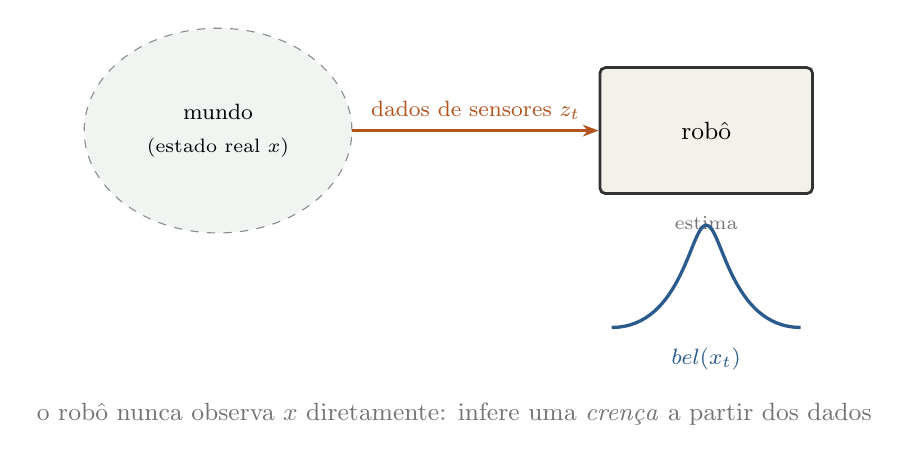
\begin{tikzpicture}[x=1cm,y=1cm]

  % mundo
  \node[draw=black!45, dashed, ellipse, minimum width=3.4cm, minimum height=2.6cm,
        fill=dgreen!8, align=center] (w) at (0,0)
       {\footnotesize mundo\\\scriptsize (estado real $x$)};

  % robô
  \node[dbox, minimum width=2.7cm, minimum height=1.6cm] (r) at (6.2,0) {\small robô};

  % dados de sensores
  \draw[dmeas, line width=1.2pt] (w.east) -- node[above, dorange, font=\footnotesize] {dados de sensores $z_t$} (r.west);

  % crença dentro do robô
  \node[below=0.15cm of r, align=center, font=\scriptsize, black!55] {estima};
  \draw[dblue, line width=1.2pt]
    (5.0,-2.5) .. controls (5.9,-2.5) and (6.0,-1.2) .. (6.2,-1.2)
               .. controls (6.4,-1.2) and (6.5,-2.5) .. (7.4,-2.5);
  \node[dblue, font=\footnotesize] at (6.2,-2.9) {$bel(x_t)$};

  \node[dlbl] at (3.0,-3.6) {o robô nunca observa $x$ diretamente: infere uma \emph{crença} a partir dos dados};

\end{tikzpicture}
\end{document}
